To illustrate the dynamic behavior of the system, sequence diagrams may be used to model the flow of interactions between different components, in order to visualize the processes involved. The following diagrams detail three of the most critical use cases in the platform.

\paragraph{Agent Creation Sequence}
The creation of a new recommender agent is a complex, asynchronous process that engages all system components. As shown in Figure~\ref{FIG:SEQ_AGENT_CREATION}, it begins when the user submits dataset files and configuration through the frontend. The backend \acs{api} validates the request and initiates a data processing pipeline that cleans invalid values, fills missing entries, removes duplicates, and normalizes ratings. 

After preprocessing, the system constructs a graph representation, ingesting users and items as nodes and interactions as edges into a FalkorDB graph, creating a reference structure for downstream tasks. With the graph in place, the backend begins training and tuning of an expert model using the processed dataset. Afterwards, the resulting model and dataset artifacts are stored, and the agent's metadata is updated to mark the process as complete. In the case of exceptions---such as failures in preprocessing, ingestion, or training---the system rolls back by deleting temporary files, model and dataset artifacts, graph data, and agent metadata to ensure consistency. Once successful, the recommender agent becomes accessible through the \acs{api}, ready for conversational recommendations and management tasks.

\newpage

\begin{figure}[Sequence Diagram for Agent Creation]{FIG:SEQ_AGENT_CREATION}{Sequence Diagram for Agent Creation.}
    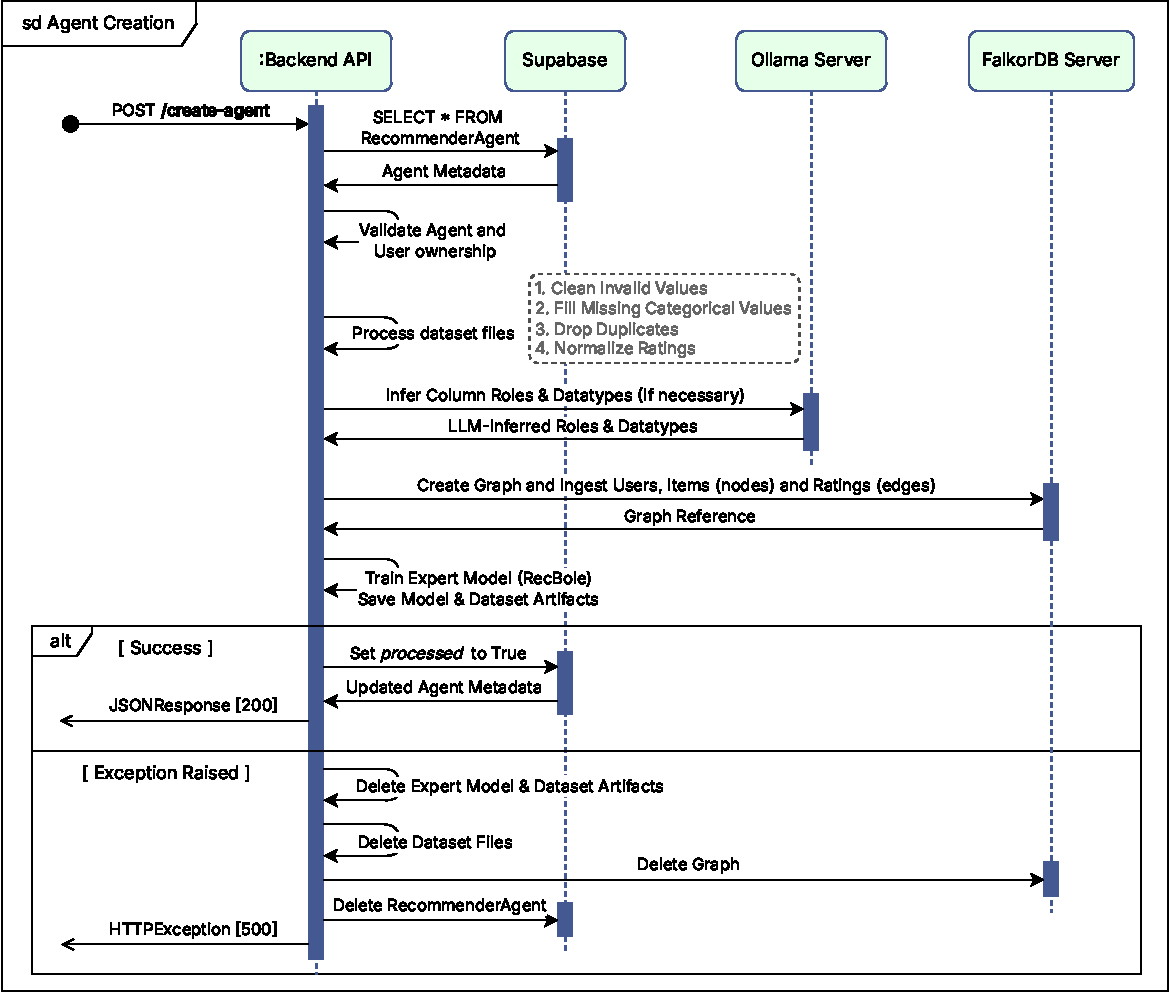
\includegraphics[width=\textwidth]{sd_agent_creation.pdf}
\end{figure}

\paragraph{Agent Chat Interaction Sequence}
A typical agent chat interaction involves a conversation between the user, the \ac{llm}, and the underlying recommendation engines. As shown in Figure~\ref{FIG:SEQ_AGENT_CHAT}, a user's message is sent to the backend, which forwards it to the LlamaIndex workflow. The workflow may use Function Calling to invoke the recommendation module (either the graph-based or expert model) to retrieve a list of recommendations and explanations, formatted into a natural language response by the \ac{llm} and streamed back to the user. Finally, each message by the user and the agent is saved in the conversation history, just as depicted in the next diagram (Figure~\ref{FIG:SEQ_OPEN_CHAT}). The internal design and implementation details of the conversational agents are discussed in the complementary research thesis \cite{MUI2ICSI-THESIS}.

\begin{figure}[Sequence Diagram for Agent Chat]{FIG:SEQ_AGENT_CHAT}{Sequence Diagram for an Agent Chat interaction.}
    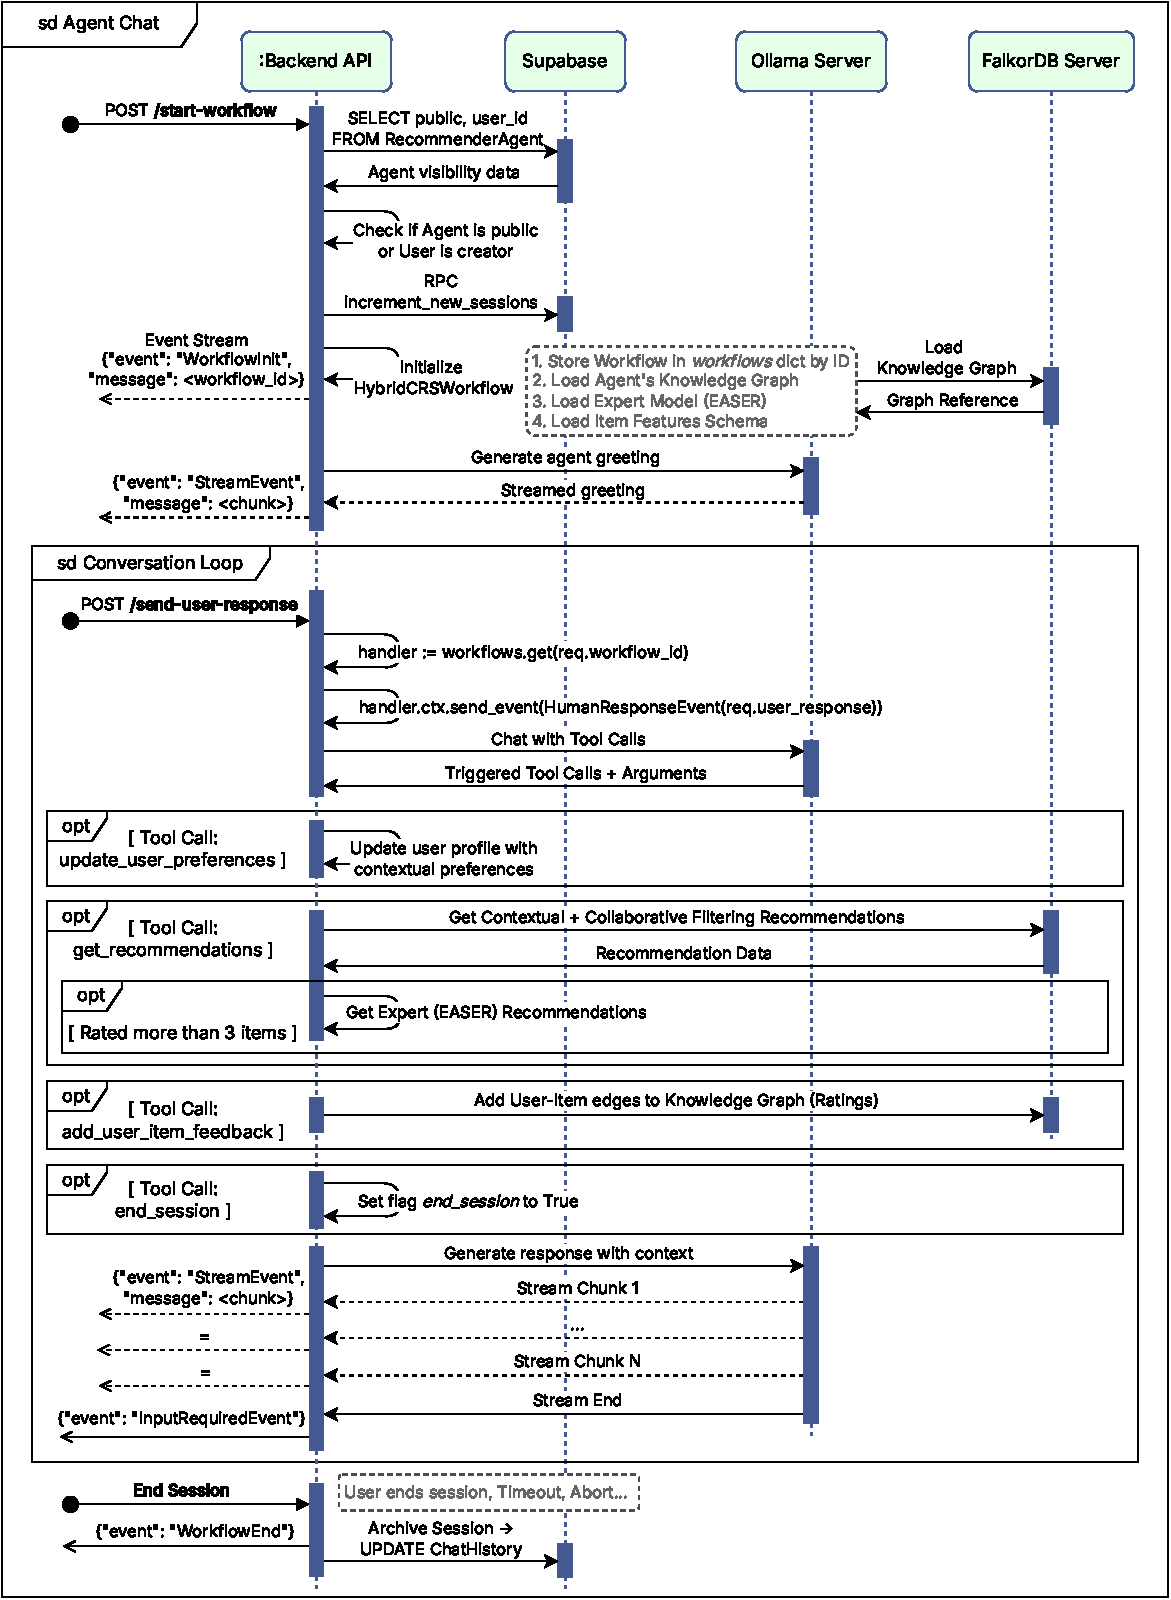
\includegraphics[width=\textwidth]{sd_agent_chat.pdf}
\end{figure}

\paragraph{Open Chat Interaction Sequence}
This interaction describes the open chat functionality, where the user interacts freely with any \ac{llm} available in the platform. The sequence diagram in Figure~\ref{FIG:SEQ_OPEN_CHAT} illustrates how the user sends a chat request to the backend, which then proxies it to the Ollama service. Any PDF attachments are processed beforehand through the \acs{api} by extracting all the text and including it in the user message. The model generates a response and streams the reply back to the user through the backend server. Finally, each message by the user and the model is saved in the conversation history, as a node in a FalkorDB graph.

\begin{figure}[Sequence Diagram for Open Chat]{FIG:SEQ_OPEN_CHAT}{Sequence Diagram for an Open Chat interaction.}
    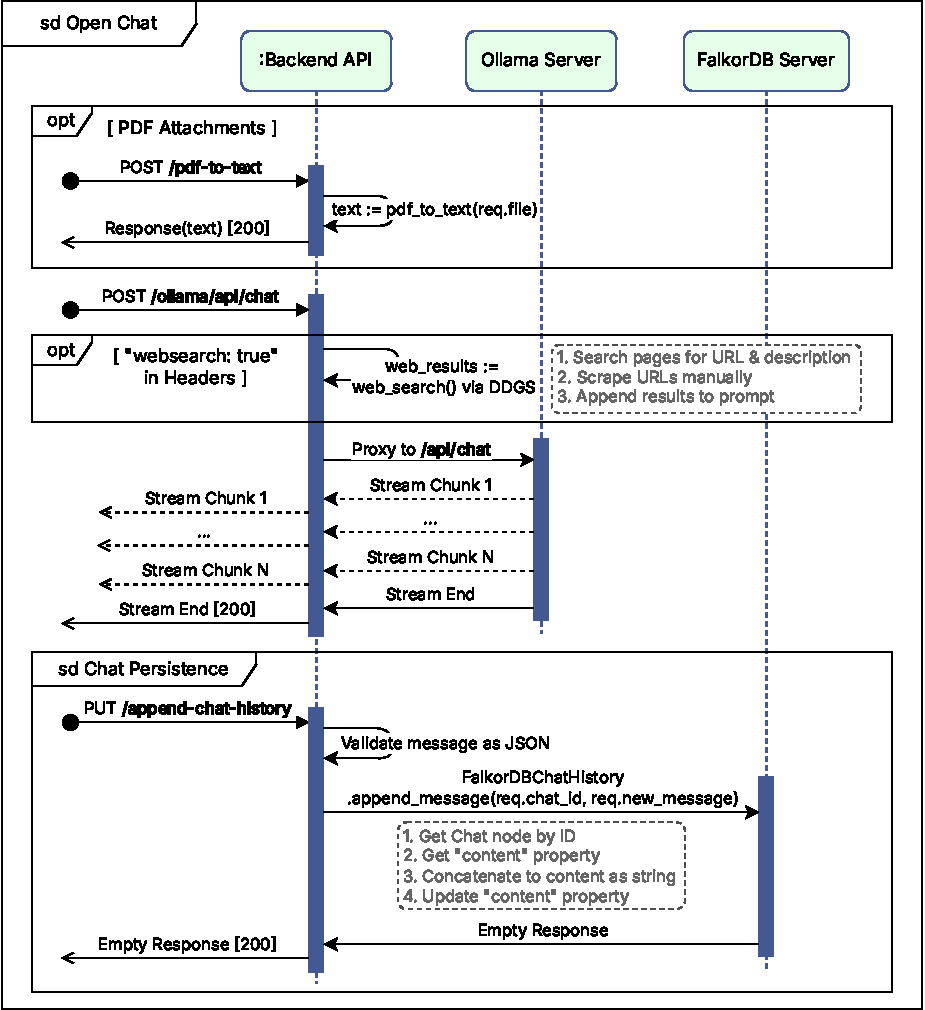
\includegraphics[width=0.8\textwidth]{sd_open_chat.pdf}
\end{figure}

\newpage